% #############################################################################
% This is Chapter 7
% !TEX root = ../main.tex
% #############################################################################
% Change the Name of the Chapter i the following line
\fancychapter{Alternative approaches to parameter-efficient transfer learning}
\label{chap:7}
\cleardoublepage
\section{Introduction}
In the previous chapters, we demonstrated the efficacy of Adapters, specifically residual Adapters, in diverse tasks related to Children's \ac{ASR}. These tasks included their uses in \ac{PETL} for children \ac{ASR} and as domain mismatch reducer for \ac{TTS} data augmentation. The success observed in these experiments has prompted a more in-depth analysis of potential alternatives to Adapters. Motivated by the literature where alternative approaches offer superior performances and more parameter-efficient solutions.
Indeed, the gowing attention towards \ac{PETL} from the research community has led the emergence of an array of novel architectures and methodologies. These alternatives extend beyond the conventional Adapters. These innovative approaches have been extensively explored in various domains such as \ac{NLP} and image processing but remain relatively unexplored in the domains of speech processing and, even more in children's \ac{ASR}.

The objective of this section is to analyse these emerging \ac{PETL} methods specifically in the context of children's \ac{ASR}. Drawing from our prior findings, which underscored the significance of fine-tuning \ac{FFN} modules, we have curated a selection of \ac{PETL} approaches designed to be integrated with \ac{FFN}. Notably, we excluded \ac{PETL} approaches centered around the \ac{MHSA} modules, such as LORA \cite{hu2022lora}, as well as any prompt-related \ac{PETL} strategies like prompt tuning \cite{lester-etal-2021-power} or prefix tunning \cite{li-liang-2021-prefix}.

This chapter starts with a in-depth presentation of the selected \ac{PETL} in order to answer the following research question: \textit{Can we further improve the parameter-efficiency with other architectures? } Each chosen methodology is thoroughly described, elucidating its underlying principles, architectural intricacies, and key characteristics conpared to the traditional Adapter. 
Following, we assess the performances of these selected \ac{PETL} methodologies  in the specific context of children's \ac{ASR}. The evaluation encompasses various dimensions, including performances compared to the full-finetuning and parameter-efficiency. By systematically benchmarking these alternative \ac{PETL} methodologies against the conventional Adapter models, our objective is to not only understand the individual strengths and limitations of these approaches but also to evaluate their relative effectiveness in tackling the specific challenges presented by children's \ac{ASR}.

\section{Exploring PETL literature alternatives}
% general introduction of the two different type of new \ac{PETL} (mention here why LORA and prompt based methods are not here) 
\subsection{Scaled Adapters}
% Explain the idea has been used in many example
Scaled or Gated Adapters extend the conventional residual Adapters by introducing a scaling mechanism to the output of the Adapter modules. The concept of scaled-Adapters was initially introduced by \cite{he2022towards} and is formally expressed as:
\begin{equation}
    adapter(x) = x + s \cdot (W_{up}(f(W_{down}g(x) + b_{down})) + b_{up})    
\end{equation}
% Tunable parameters
Here, $s \in \mathbb{R}$ is a tunable scalar hyperparameter. Notably, some research has proposed the to learn directly this scalar value during training as a gate mechanism \cite{mao-etal-2022-unipelt}. The intuition behind this approach is to allow the network to gradually learn to assign weights to the target domain, achieving more fine-grained control of the Adapter activation or deactivation. The scaled learning process facilitates the regulation of contributions from the Adapters from differents layers, enabling the model to adapt and refine its responses based on the specific characteristics of the data encountered during training.
% Experimental setup
Within the context of our experiments, we decided to use a trainable scalar associated to each Adapter modules. This scaling parameters and all Adapter modules were optimised through a 30 epochs training using a learning rate of $8 \times 10^{-4}$.

\subsection{Convolution based Adapters}
% CNN make sense for speech
Convolutional Neural Networks have been widely recognised for their effectiveness in exploiting local information, particularly for computer vision tasks. These networks learn shared kernels based on position within localised windows, giving them the ability to capture features such as edges and shapes. This characteristic has also been demonstrated in the field of speech-related tasks, as demonstrated by the success of the Conformer architecture \cite{gulati2020conformer}.

%Then CNN in Adapter is a normal step
As a result of this success, \acp{CNN} have been naturaly incorporated into Adapter modules. This strategic fusion enables Adapters to leverage the spatial processing capabilities inherent in convolutional modules, thereby enhancing their capacity to capture and adapt to different patterns present in the data. The initial approach involved using \acp{CNN} as feature extractors, in conjunction with a linear transformation, as detailed by \cite{yang23p_interspeech}, we denoted this approach as Conv-Adapter. We experimented two version of Conv-Adapters, where a 1-dimensional \ac{CNN} is used as replacement of either the first of second linear of the traditional Adapters. More formally, the \textit{$\text{Conv-Adapter}_{down}$} expressed as followed:
\begin{equation}
    \text{Conv-adapter}_{Down}(x) = x + (W_{up}(\text{CNN}_{1D}(x))+ b_{up})
\end{equation}
While \textit{$\text{Conv-Adapter}_{up}$} is defined as:
\begin{equation}
    \text{Conv-adapter}_{up}(x) = x + \text{CNN}_{1D}(W_{down}(x)+ b_{down})
\end{equation}
We also investigated, the \cite{muthuchamyselvaraj23_interspeech} Conv-Adapter where the \ac{CNN} is integrated in between the Up and Down projection of the traditional Adapter, denoted \textit{$\text{Conv-Adapter}_{Middle}$}, mathematically expressed as:
\begin{equation}
    \text{Conv-adapter}_{Middle}(x) = x + W_{up}(\text{CNN}_{1D}(W_{down}(x)+ b_{down})+ b_{up})
\end{equation}

\begin{figure}
    \begin{center}
        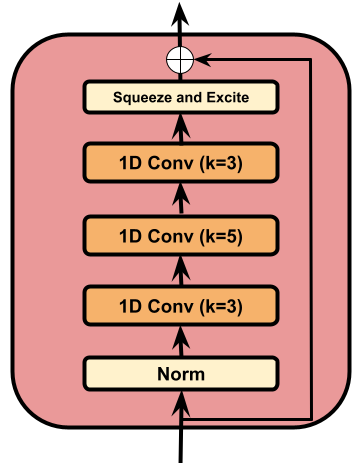
\includegraphics[scale=0.4]{imgs/ConvPass.png}
        \caption{Th architecture of the ConvPass adapter. $k$ is the kernel size of the 1D convolution. All Convoluation are depth-wise convolution.}
        \label{fig:convpass}
    \end{center}
\end{figure}

% Adapter fully CNN based
An alternative approach involves the use of a fully \ac{CNN}-based Adapter known as ConvPass, which has demonstrated effectiveness in computer vision tasks \cite{jie2022convolutional}. Diverging from conventional Adapters and the previously mentioned Conv-Adapter, ConvPass distinguishes itself by the removal of the up and down linear layers, replaced instead by three \ac{CNN} layers. In \cite{jie2022convolutional}, these layers comprise a $1 \times 1$ convolution, followed by a $3 \times 3$ convolution, and another $1 \times 1$ convolution. Notably, \ac{GELU} activation functions are interposed between these convolutional layers.

For speech-related tasks, a comparable approach was introduced by \cite{li2023evaluating}. The speech-specific ConvPass, illustrated in Figure \ref{fig:convpass}, incorporates a layer normalisation layer, followed by three lightweight 1-dimensional \ac{CNN} layers with kernel sizes of 3, 5, and 3, respectively. Additionally, a squeeze and excite module is integrated into the architecture. The squeeze and excite module, as proposed by \cite{hu2018squeeze}, facilitates feature recalibration. It consists of a global pooling operation, followed by a linear layer, a \ac{ReLU} activation, a second linear layer, and concludes with a Sigmoid activation.

During our experiments, all Conv-Adapters and ConvPass configurations were trained for 30 epochs with a learning rate of $8 \times 10^{-4}$.


\subsection{BitFit}
Bias-Term Fine-Tuning, known as BitFit, is a \ac{PETL} method introduced by \cite{ben-zaken-etal-2022-bitfit} for NLP tasks. The main idea behind BitFit is to fine-tune only the bias terms and the task-specific classification layer while keeping the rest of the model frozen. This approach aims to achieve efficient fine-tuning with reduced computational requirements in a similar way as our partial fine-tuning experiments in chapter \ref{chap:4}. The fine-tuning of bias terms can be seen as introducing a task-specific shift to the token representations.

%Advantages of Bitfit
The authors highlight three key properties of BitFit. Firstly, it matches of a fully fine-tuned model, showcasing its ability to maintain comparable results while significantly reducing the number of parameters to be trained. Secondly, BitFit is designed to adapt to tasks arriving sequentially, eliminating the need for simultaneous access to all datasets. This adaptability enhances the model's versatility in handling diverse tasks with varying data distributions over time. Thirdly, BitFit exhibits parameter efficiency by fine-tuning only a small subset of the model's parameters.

%Experimental setup
In our experiment, the pre-trained model and children's \ac{ASR} task shared the same output dimensions and character encoding. In consequence, we excluded the fine-tuning of the task-specific classification layer. The training process consisted of 30 epochs with a learning rate of $8 \times 10^{-4}$.

\subsection{Scale and Shift features}
% Define SSF
\ac{SSF} was introduced an \ac{PETL} alternative approach by Lian and al. \cite{lian2022scaling} for image classification. The primary objective of SSF is to establish a generalised method for efficient model fine-tuning without the introduction of task-specific inference parameters. Drawing inspiration from feature modulation techniques such as \cite{wu2018group,huang2017arbitrary}, the \ac{SSF} method modulate deep features extracted by a pre-trained model by scaling and shifting them to match the distribution of a target dataset. 
The intuition behind \ac{SSF} comes from the inherent disparities in data distributions between upstream and downstream datasets. Directly applying model weights trained on an upstream dataset to a downstream dataset frequently leads to a performance degradation due to the disparities between the two datasets \cite{sun2016return}. The \ac{SSF} method addresses this challenge by introducing scale $\gamma$ and shift $\beta$ parameters, which could be considered as the variance and mean used to modulate the features extracted from the pre-trained model. This modulation ensures that the adapted features align with the characteristics of the upstream dataset. Formally, given an input $x$, the modulated output $y$ is calculated by:
\begin{align}
    y = \gamma \odot x + \beta
\end{align}

Notably, the scale and shift parameters in \ac{SSF} remain independent on any input and have a unified learnable parameter-space for different tasks. Another noteworthy advantage of \ac{SSF} is its reliance on linear transformations, which can be seamlessly merged into the original pre-trained weights during model re-parameterization in the inference phase. This integration avoid the need for additional parameters removing the extra-computation time of other \ac{PETL} such as Adapters.

% How to put it in a model
In practical terms, \ac{SSF} are introduced after each modules within the Conformer architecutre (\acp{FFN}, \ac{MHSA} and Convolution modules). In the original paper, they also finetuned the Head-layers as the task is a image classification task, as our both upstream and downstream tasks, respectively adult and children \ac{ASR}, share the same output dimension and character encoding, we do not finetune this extra layer and only use the \ac{SSF} method. 

%Experimental setup
In practice, the \ac{SSF} modulation is integrated after each operations of the neural network. For our experiments, each operations corespond the different modules within the Conformer architecture, specifically the \acp{FFN}, \ac{MHSA} and Convolution modules. It is noteworthy that, in the original paper, the authors also fine-tuned an Head-layer, as the output of the upstream and downstream image classification tasks are different. However, in our experiment, both the upstream and downstream tasks involve English \ac{ASR} with shared output dimensions and characters encoding. Therefore,we did not include the head-layer fine-tuning and exclusively employed the \ac{SSF} method. Our training compromise 30 epochs with a learning rate of $8\cdot10^{-4}$.


\subsection{AdapterBias}
\begin{figure}
    \begin{center}
        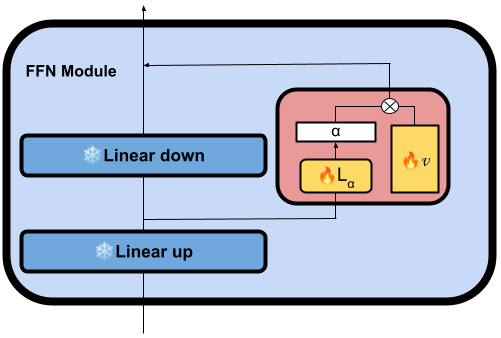
\includegraphics[scale=0.4]{imgs/AdapterBias.png}
        \caption{ AdapterBias, consisting of a linear layer $L_\alpha$ and a vector $\mathcal{V}$, is added after the second feed-forward layer only in each FFN module.}
        \label{fig:AdapterBias}
    \end{center}
\end{figure}
% Link to Bitfit
Following the success of BitFit \cite{ben-zaken-etal-2022-bitfit}, which aims to introduce task-specific shifts to each output representation by selectively fine-tuning only the bias terms of a pre-trained model, recent research has suggested that certain tokens may hold more significance than others for specific tasks. While BitFit uniformly applies the same shift across all tokens regardless of their relevance to the task, \cite{fu-etal-2022-adapterbias} proposes AdapterBias to address this limitation.

% What is AdapterBias
AdapterBias comprises two essential modules: a vector $\mathcal{V}$ and a linear layer $L_\alpha$. The vector $\mathcal{V}$ represents a task-specific shift added to the output of each \ac{FFN} modules, acknowledging that tokens more closely related to the task should be assigned to larger representation shifts than others. On the other hand, the linear layer $L_\alpha$ generates a token-dependent weight vector $\alpha = [\alpha_1, \alpha_2, ..., \alpha_m]^T$, where $\alpha_i$ is the weight associated with the representation shift of the $i^{th}$ token. By applying these token-specific weights to the task-specific representation shift $\mathcal{V}$, AdapterBias focuses on tokens which are more crucial to the task, allowing efficient and fine adaptation to various downstream tasks.

The output of AdapterBias is defined as the bias (B), represented as the outer product of $\mathcal{V}$ and the learned weights vector $\alpha$. Mathematically, the output of AdapterBias is expressed as follows:

\begin{equation}
    B = \mathcal{V} \otimes \alpha^T    
\end{equation}

Here, \(\otimes\) denotes the element-wise multiplication of the task-specific shift vector \(\mathcal{V}\) and the token-dependent weight vector \(\alpha\).
% Experimental seting
In our experimental setup, we conducted the training for AdapterBias by integrating them into the second linear layer of each of the two \ac{FFN} modules within the Conformer architecture. We trained AdapterBias for 30 epochs, employing a learning rate of $8 \times 10^{-4}$.

\subsection{Results of the different PETL methods}

\begin{figure}
    \begin{center}
        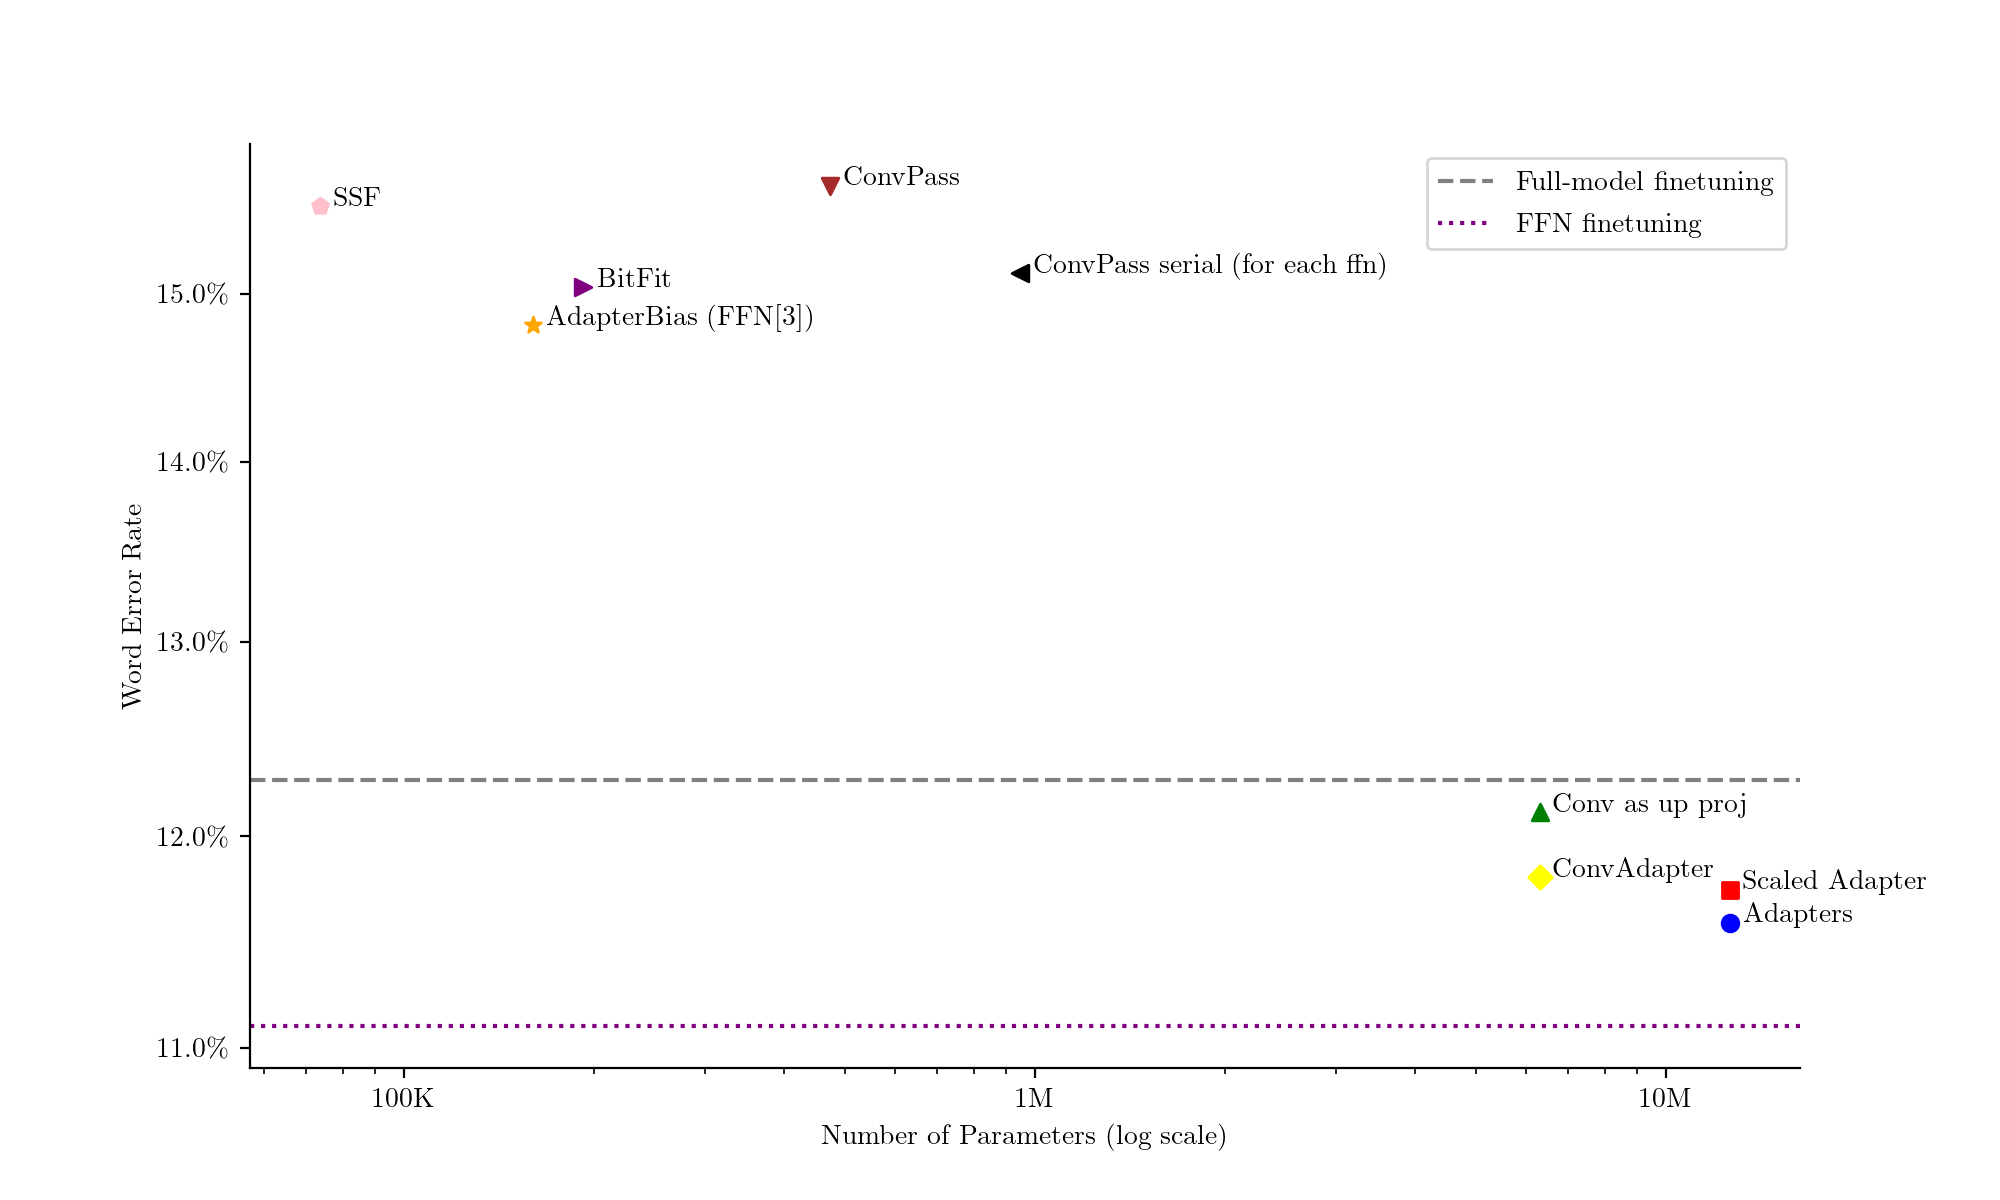
\includegraphics[width=\textwidth]{imgs/Adapter_compare_withoutWide.png}
        \caption{Different paramter efficent procedure for children ASR in Conformer model}
        \label{fig:adapter_compared_withoutWide}
    \end{center}
\end{figure}
\begin{table}
    \centering
    \begin{tabular}{lccc}
        \toprule
        \textbf{Method} & \textbf{WER $\downarrow$} & \textbf{Trained Parameters} \\
        \midrule
        Adapter & \textbf{11.58\%} & 12.6M \\
        Scaled Adapter & 11.74\% & 12.6M \\
        ConvAdapter(Down) & 12.03\% & 6.4M \\
        ConvAdapter (Middle) & 11.62\% & 12.7M \\
        ConvAdapter (Up) & 11.78\% & 6.4M \\
        ConvPass & 15.13\% & 946.2K \\
        BitFit & 15.04\% & 192K \\
        SSF & 15.55\% & 73.7K \\
        AdapterBias & 14.81\% & 159.8K \\
        \bottomrule
    \end{tabular}
    \caption{Performances of the different PETL alternatives}
    \label{tab:PETL_alternatives}
\end{table}
% Adapter and Scaled Adapter
The results of various \ac{PETL} methods are summarised in Table \ref{tab:PETL_alternatives}. Notably, the traditional residual Adapter approach using the \ac{TPA} configuration emerges as the most effective, achieving a 11.58\% \ac{WER} with 12.6 million parameters. The Scaled Adapter method exhibits a slightly reduced \ac{WER} performance at 11.74\%, while maintaining the same parameter count of 12.6 million.

%ConvAdapter and ConvPass
Turning attention to convolution-based Adapters, the replacement of either linear layer ($W_{down}$ and $W_{up}$) results in decreased performance, yielding WERs of 12.02\% and 11.78\%, respectively, using both 6.4 million parameters. Interestingly, introducing a convolutional layer between these two linear layers proves to be the best-performing convolutional system, approaching the scores of the regular Adapter with 11.62\% \ac{WER} and using a slightly increased amount of parameters of 12.7 million. It is noteworthy that all these Conv-Adapter setups and the Scaled Adapters approach continue to outperform the fine-tuning of the entire model and are therefore valuable appraoches for children's \ac{ASR} \ac{PETL}.
On the other hand, the ConvPass method, where all linear layers of the Adapter are replaced by convolution layers, does not surpass the full fine-tuning, yielding a \ac{WER} of 15.13\% with 946.2 thousand parameters.

% Bitfit, SSF and AdapterBias
Moving to bias shift methods, including BitFit, \ac{SSF}, and AdapterBias, these approaches underperform compared to the entire model fine-tuning, with respective \acp{WER} of 15.04\%, 15.55\%, and 14.81\%. However, it's important to note that these methods use significantly fewer parameters, with 192, 73.7, and 159.8 thousand parameters, respectively.

% Summary
In summary, the traditional residual Adapter emerges as the most effective \ac{PETL} approach for children's \ac{ASR}. This finding aligns with recent research, as highlighted in studies such as \cite{li2023evaluating} and \cite{cappellazzo2023parameter}, which also affirm the superior performance of Adapters in \ac{PETL} for \ac{ASR} tasks. Moreover, our findings highlight a noticeable trade-off between the number of parameters and the \ac{WER}. Specifically, approaches employing fewer than a million parameters do not exhibit comparable performances to entire model fine-tuning, as illustrated explicitly in Figure \ref{fig:adapter_compared_withoutWide}. This trade-off emphasises the need for more research on the development of \ac{PETL} methods that can effectively use fewer parameters while simultaneously maintaining or enhancing performance in the domain of children's \ac{ASR}.

\section{Advancement in Adapters: Introducing Shared-Adapters}
\subsection{Motivation}
% Goal PETL- Good score, small |param|
The primary objective of \ac{PETL} is to either maintain or surpass the performance achieved through full fine-tuning of a pre-trained model, while minimising the number of parameters employed during training. In previous section, the efficiency of residual Adapters has been underscored. Remarkably, using only 10\% of the total number of parameters compared to the fine-tuning of the entire model, these residual Adapters exhibit superior performances in the context of children's \ac{ASR}. In addition, our experiments highlighted the drawback of overparameterisation present in Transformer-based models.

% FFN redundancy
Leveraging this understanding, we propose a novel \ac{PETL} methodology developed on the concept of sharing one residual Adapters across alll layers. The inspiration for this approach draws from the insights provided by the work of \cite{pires2023one}, which focus on the \ac{FFN} modules. Despite representing a significant proportion of the model's parameters, the \ac{FFN} was identified as highly redundant. This affirmation is confirmed by the work of \cite{geva2020transformer}, which  establishes a connection between the \ac{FFN} and attention mechanisms by proposing that the \ac{FFN} corresponds to learnable key-value memories. In this conceptualisation, the weights of the first layer of the \ac{FFN} represent the keys, while those of the second layer correspond to the values. These keys are proficient at capturing salient patterns at each layer. Interestingly, they observed that the classes of patterns tend to overlap between neighboring layers, indicating redundancy in the representation. This observation underscores the potential for optimising \ac{PETL} methods by addressing and mitigating redundancy within \ac{FFN} modules, ultimately contributing to more parameter-efficient transfer learning processes.

% Shared FFN work
Building upon this observation, \cite{pires2023one} modified the conventional Transformer architecture by sharing and dropping the \ac{FFN} across different layers. Their investigation confirms the substantial degree of redundancy between the \acp{FFN} of the Encoder and Decoder components. Consequently, they successfully eliminate the Decoder \ac{FFN} while sharing a single \ac{FFN} across the Encoder, achieving a noteworthy reduction in model parameters without significant compromise to accuracy.

Formally, with $N_{enc}$ denoting the number of Encoder layers, the sharing of the \ac{FFN} modules in the Encoder can be expressed as follows:

\begin{equation}
    \text{FFN}_{i}^{enc}(.) \stackrel{\text{tied}}{=} \text{FFN}^{enc}_{all}(.) , \forall i: 1 \leq i \leq N_{enc}
\end{equation}

%Shared Adapter motivation
In light of the success observed with the shared \ac{FFN} in the Encoder, we hypothesise that the presence of redundancy within the \ac{FFN} might lead to a similar redundancy issue when employing one Adapter per \ac{FFN} layer. In other words, employing separate Adapters plugged to redundant \ac{FFN} modules for different layers might also exhibit redundancy. To address this concern, we introduced the \textit{Shared Adapter} approach, wherein a single residual Adapter is used across all layers as shown in figure \ref{fig:adapter_compared}. This approach aims to use the redundancy present in \ac{FFN} layers modules to reduce the total amount of parameters used in Adapter-transfer. The formal expression of the Shared Adapter is presented as follows:

\begin{equation}
    \text{Adapter}_{i}(.) \stackrel{\text{tied}}{=} \text{Shared-Adapter}_{all}(.) , \forall i: 1 \leq i \leq N_{enc}
\end{equation}

% Compared to traditional adapter + Hidden dimension + Number of hours
In order to evaluate our proposed approach, our initial focus is on comparing the Shared-Adapter configuration with full fine-tuning and the Traditional Adapter. Subsequently, we vary the hidden dimension of the Shared-Adapter to assess how the number of parameters and the hidden dimension influence the performances of the different Shared-Adapters. This comprehensive analysis aims to provide insights into the effectiveness of Shared-Adapters across various scenarios and configurations. Finally, we assess the robustness of both Traditional and Shared-Adapters by examining their performances under different amounts of training data. The aim is to evaluate how these methods perform in low and very low-resource scenarios.

\subsection{Experimental setup}
\begin{figure}[t]
    \centering
    \subfigure[Shared-Adapter setup in a Conformer model]{\label{fig:Shared_adapter}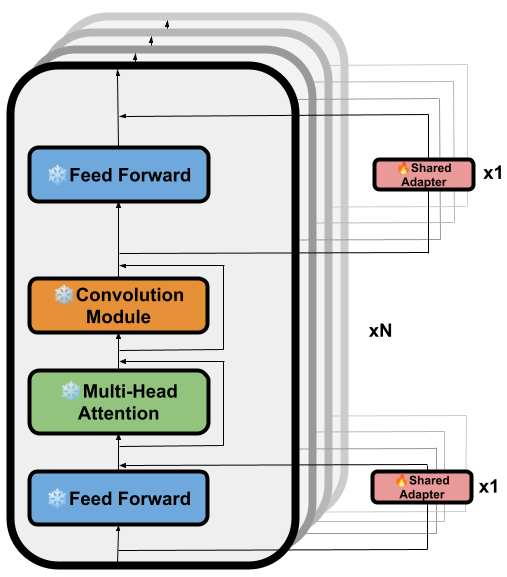
\includegraphics[width=0.45\textwidth]{imgs/Shared_Adapters.png}}
    \subfigure[Extremly Shared-Adapter setup in a Conformer model]{\label{fig:extrem_adapter}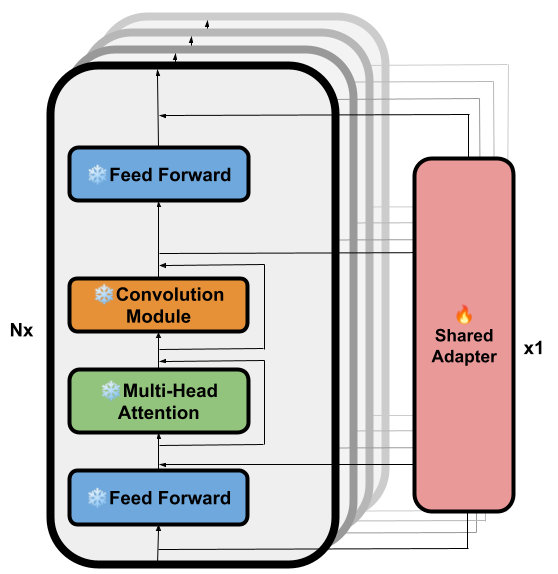
\includegraphics[width=0.48\textwidth]{imgs/Extreme_shared_adapter.png}}
    \caption{Overview of the Shared Adapters configurations}
\end{figure}


In our analysis, we focus on evaluating the performance of the Shared-Adapter using the same setting as the \ac{TPA} configuration for traditional Adapters, as the \ac{TPA} configuration was found to be the most effective in Conformer models. Specifically, we assess the Shared-Adapter within a Conformer \ac{ASR} model, where the two Shared-Adapters are directly integrated into the two \ac{FFN} modules at each layer as shown in Figure \ref{fig:Shared_adapter}.  The hidden dimension of the Shared-Adapters is set to 512. The Conformer model comprises 12 Conformer layers followed by 6 Transformer layers, and for this experiment, we exclusively evaluate the Shared-Adapter in the Encoder.
To quantify the reduction of the number of parameters used in the Shared-Adapter compared to the traditional Adapter, the following formula is used:
\begin{equation}
    \text{Number of Parameters in Shared-Adapter} = \frac{\text{Number of Parameters of all traditional Adapters}}{\text{Number of Layers}}
\end{equation}

In addition, we propose an extension of the Shared-Adapters concept within the \ac{TPA} configuration. This novel approach, called \textit{Extreme Shared-Adapter} involves using a single Adapter for all \ac{FFN} modules. This configuration has the potential to further reduce the number of parameters by half compared to the use of two Shared-Adapters in the \ac{TPA} setup. This Extreme Shared-Adapter configuration is presented in Figure \ref{fig:extrem_adapter}. This exploration aims to test the limits of the parameter efficiency and accuracy balance of our approach within the context of children's ASR. For training all our different models, we use 30 epochs with a learning rate set to $8 \times 10^{-4}$.

For our experimental setup, while the traditional Adapter use approximately 12.6 million parameters, the number of parameters employed by the Shared-Adapter transfer is approximately 1.1 million and  the Extreme Shared-Adapter uses only 527.9 thousand parameters. This represents a substantial reduction, as the Shared-Adapter and Extreme Shared-Adapter configurations use only 8\% and 3\%, respectively, of the number of parameters of the traditional Adapters setup. Moreover, considering that the traditional Adapter already represents approximately 10\% of the total parameters used in the entire model fine-tuning, the Shared-Adapter and Extreme Shared-Adapter configurations use only 1\% and 0.5\%, respectively, of the trainable parameters when compared to the entire model fine-tuning. This reduction in the number of parameters highlights the parameter efficiency gains achieved by these novel configurations.

\subsection{Results}
\subsubsection{Shared-Adapter compared to other PETL methodologies}
\begin{figure}[t]
    \begin{center}
        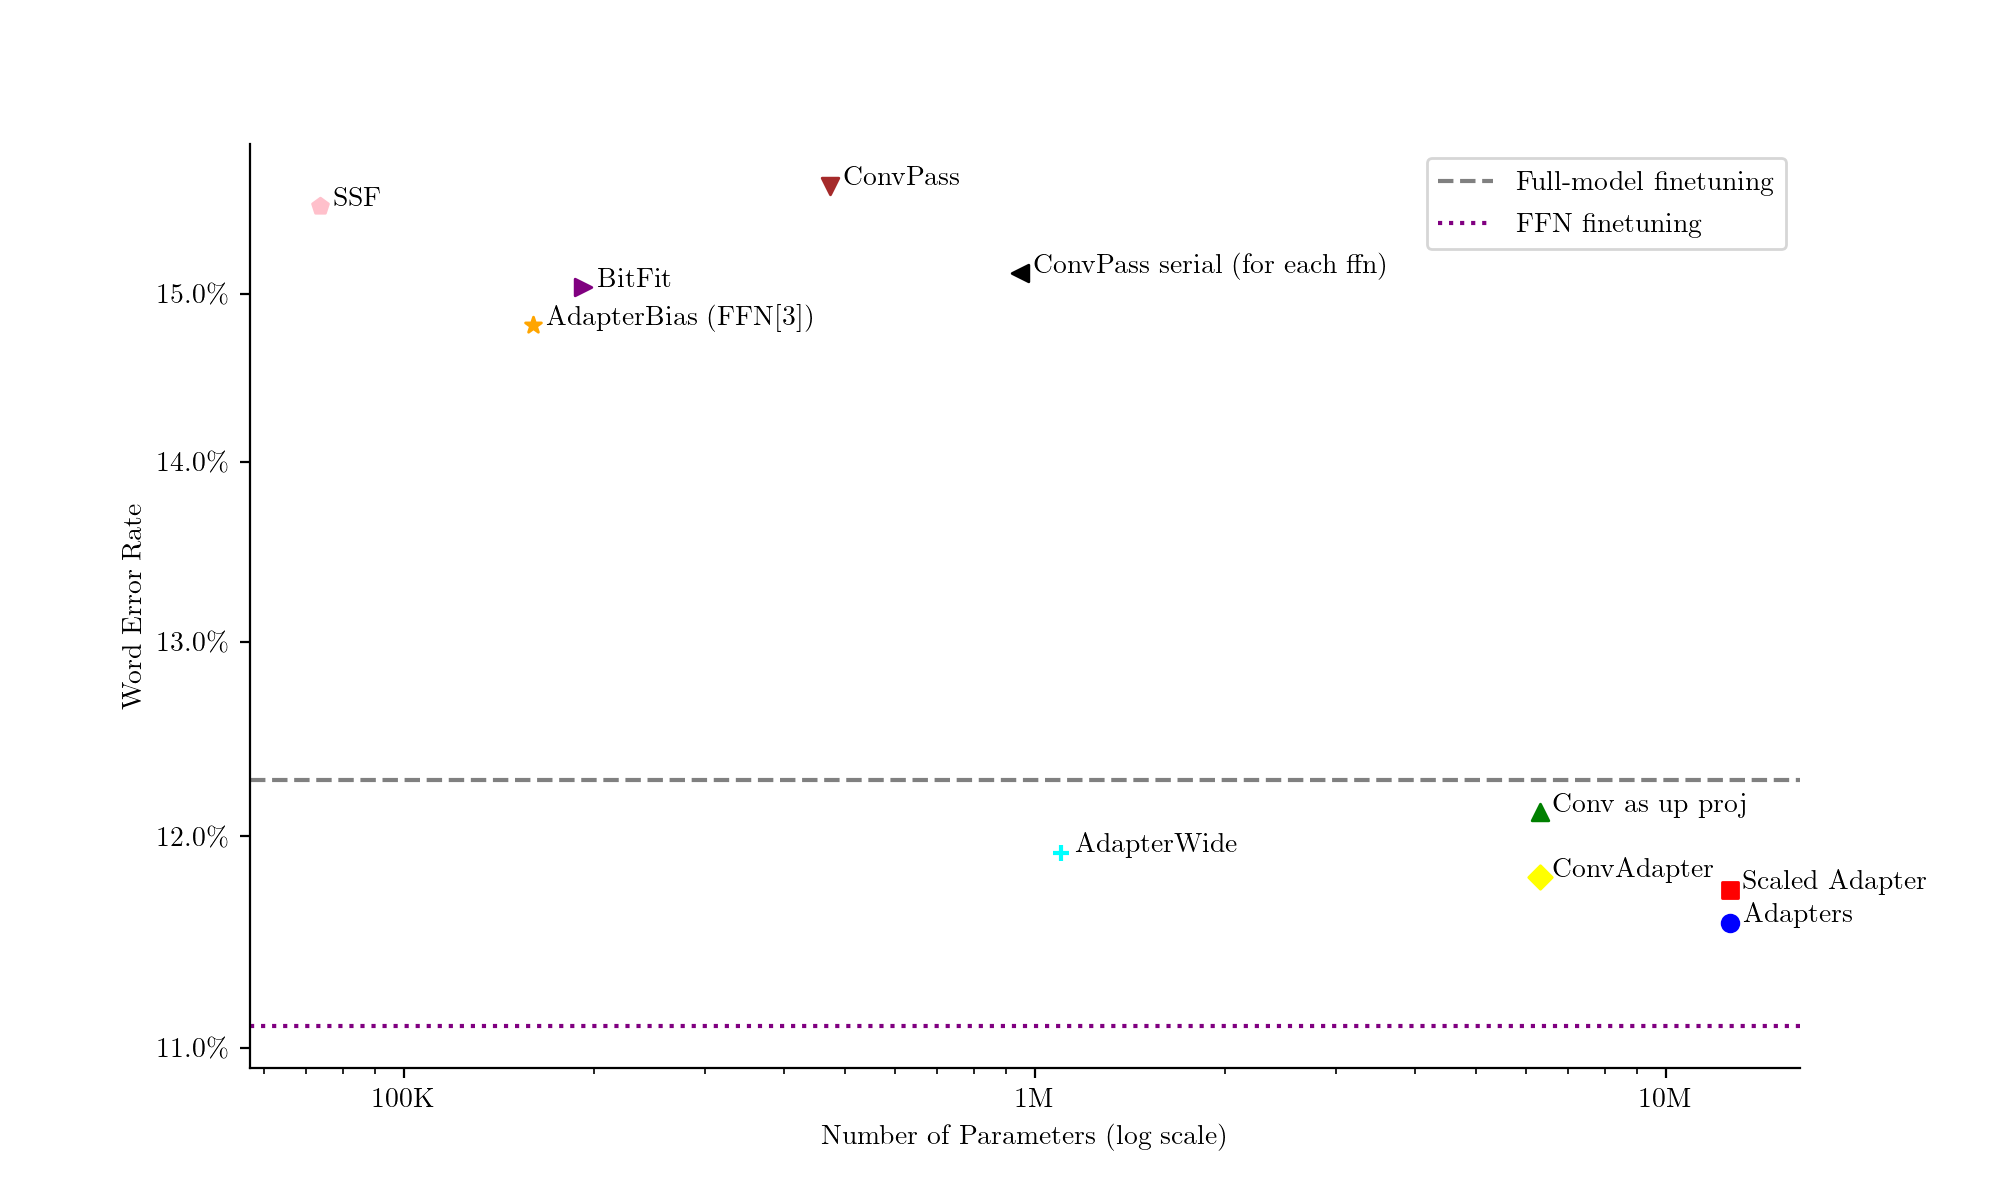
\includegraphics[width=\textwidth]{imgs/Adapters_compare.png}
        \caption{Different paramter efficent procedure for children ASR in conformer model with shared-Adapters}
        \label{fig:adapter_compared}
    \end{center}
\end{figure}


In our comparative analysis, we systematically evaluate the efficacy of our proposed Shared-Adapter configuration against established \ac{PETL} methods, as illustrated in Figure \ref{fig:adapter_compared}. The observed outcomes underscore the notable performance of the Shared-Adapter, particularly in achieving a remarkable balance between parameter efficiency and accuracy. Notably, the Shared-Adapter outperforms the full-model fine-tuning performance while using a only 1\% of the entire model number of parameters. Although the Extreme Shared-Adapter exhibits a marginal degradation, surpassing the \ac{WER} of the entire model fine-tuning, it still outperforms alternative methods such as ConvPass and BitFit by a large marging. These findings substantiate the efficiency of the Shared-Adapter as a novel parameter-efficient strategy, demonstrating a superior balance in comparison to existant methodologies. The precise results of the Shared-Adapter and Extreme Shared-Adapter are presented in Table \ref{tab:shared_adapter_results}.

\subsubsection{Evaluating the parameter influence on Shared-Adapter}
\begin{table}[ht]
    \centering
    \begin{tabular}{l c c c}
        \hline
        \textbf{Configuration} & \textbf{WER $\downarrow$} & \textbf{Trained Params} \\
        \hline
        Full Fine-tuning & 12.28\% & 109.1M \\ \hline
        Traditional Adapter 512 & \textbf{11.58\%} & 12.6M \\ \hline
        Shared-Adapter 128 & 12.74\% & 265.5K \\
        Shared-Adapter 256 & 12.34\% & 527.9K \\
        Shared-Adapter 512 & 11.92\% & 1.1M \\
        Shared-Adapter 1024 & 11.90\% & 2.1M \\
        Shared-Adapter 2048 & 11.86\% & 4.2M \\
        Shared-Adapter 4096 & \textbf{11.83\%} & 8.4M \\
        Shared-Adapter 6144 & 11.88\% & 12.6M \\ \hline
        Extreme Shared-Adapter  512& 12.31\% & 526.3K \\ \hline
    \end{tabular}
    \caption{WER and Parameters for different Shared-Adapter hidden dimension}
    \label{tab:shared_adapter_results}
\end{table}


The results in Table \ref{tab:shared_adapter_results} present the performances of different configurations of the Shared-Adapter model with varying hidden dimensions compared to Traditional Adpater and full model fine-tuning. As mentioned in previon section, Shared-Adapter and Extreme Shared-Adapter highlight remarkable performances compared to Traditional Adpaters and the full model fine-tuning. Additionally, as we decrease the hidden dimension to 128, the WER increases slightly to 12.74\% \ac{WER}, with a reduction in the number of trained parameters to 265.5K. Interestingly, as the hidden dimension increases from 128 to 4096, the \ac{WER} consistently decreases. In particular, the Shared-Adapter with a hidden dimension of 4096 exhibits the best performance, achieving a \ac{WER} of 11.83\%, with a larger parameter count of 8.4M. 
However, as we push the hidden dimension further to 6144, equivalent to the parameter count in Traditional Adapters, the performance start to degrade. We also observed, a score drop compared to the Traditional Adapters setup. This decline and drop of performance suggests a tipping point where the model's capacity to effectively learn becomes challenged by the heightened complexity associated with a larger hidden dimension. 

%The results suggest that increasing the hidden dimension in the Shared-Adapter model generally improves its performance in terms of \ac{WER}, reaching a notable best performance at hidden dimension of 4096 . However, this improvement comes at the cost of a substantial increase in the number of trained parameters. Thefore, our results underscore the nuanced relationship between the hidden dimension, model performance, and the associated number of parameters where the hidden-dimension need to be carefully selected. 

\subsubsection{Low resource and extremly low resource scenarios robustness}
\label{sec:hours_PETL}
\begin{table}[ht]
    \centering
    \begin{tabular}{l c c c}
        \hline
        Number of hours & Fine-tune (109.1M) & TPA Adapter (12.6M) & Shared-Adapter (1.1M) \\
        \hline
        1h & 16.24\% & 16.51\% & 17.20\% \\
        10h & 14.00\% & 14.05\% & 14.28\% \\
        20h & 13.43\% & 13.30\% & 13.52\% \\
        50h & 12.94\% & 12.40\% & 12.57\% \\
        All (\~113h) & 12.28\% & 11.58\% & 11.92\% \\
        \hline
    \end{tabular}
    \caption{WER for different training durations for the full model fine-tune, TPA Adapter, and Shared-Adapter}
    \label{tab:training_duration_results}
\end{table}

To evaluate the efficacy of Adapter transfer and the Shared-Adapter in low and extremely low-resource settings, we present the results in Table \ref{tab:training_duration_results}, highlighting the impact of training duration on model performance. Three models are considered: Full model fine-tuning, Traditional Adapters using the \ac{TPA} configuration, and Shared-Adapter, also employing a \ac{TPA} configuration with one Shared-Adapter per \ac{FFN} module. We examine scenarios with 50 and 20 hours as low-resource settings and extremely low-resource scenarios with only 10 and 1 hour for training.

For full model fine-tuning, the \ac{WER} ranges from 16.24\% with 1 hour of training to 12.28\% with the entire training set (approximately 113 hours). In parallel, Traditional Adapters show a \ac{WER} reduction from 16.51\% to 11.58\% across the same durations. Notably, in extremely low-resource scenarios, Adapters and full transfer learning yield comparable results. However, Adapters start to outperform fine-tuning when the training duration exceeds 20 hours, reaffirming the efficiency of Adapter transfer for children's \ac{ASR}.

The Shared-Adapter model exhibits competitive performances, with a \ac{WER} decrease from 17.20\% to a notable 11.92\% as training duration extends. This establishes Shared-Adapter as a robust \ac{PETL} approach even in low-resource and extremely low-resource scenarios of children's speech.

\section{Summary and discussion}
% Summary
In this chapter we addressed to the following research question: \textit{Can we further improve the parameter-efficiency with other architectures?}. The comprehensive evaluation of various parameter-efficient transfer learning alternatives from the existing literature revealed that these alternatives did not surpass the performance achieved by traditional Adapter modules. Our results on children's \ac{ASR} highlighted the presence of a tradeoff between accuracy and parameter efficiency.

Crucially, the optimal balance was observed when \ac{PETL} methods used approximately 10\% of the total parameters in the pre-trained model. This parameter-efficient configuration consistently resulted in \ac{WER} scores below those obtained through the full-model fine-tuning. However, reducing the proportion of parameters trained to less than 10\% of the enitre model led to a notable deterioration in \ac{WER} scores, underlining the tradeoff between efficiency gains and preservation of accuracy in children's \ac{ASR} systems.


Additionally, we introduced a novel \ac{PETL} approach, the Shared-Adapter. Leveraging the inherent redundancy of \ac{FFN} modules in between in the different Transformer layers. Our experimental evaluations demonstrated that Shared-Adapters represent a breakthrough in parameter efficiency while maintaining high accuracy in children's \ac{ASR}. Notably, while conventional \ac{PETL} methods typically required around 10\% of the total model parameters, Shared-Adapters excelled by achieving comparable accuracy with only 1\% of the parameters. Pushing the boundaries even further, we explored the extreme scenario of using the Extreme Shared-Adapters configuration with a mere 0.5\% of the model's total parameters, yet still achieving performance levels similar to full-model fine-tuning. Our approach eliminates the need of the aforementioned tradeoff, offering a pathway to obtain superior parameter efficiency without compromising accuracy.

% Discussion
The remarkable success of the Shared-Adapter approach underscores the significant redundancy of the \ac{FFN} modules across different layers. This new understanding is pivotal for advancing the development of more efficient, computationally compact \ac{ASR} models. Future research directions could explore the creation of a novel Transformer architecture designed to address the observed redundancy, providing an architecture that is inherently more easy to fine-tuning for children's \ac{ASR} or even in speaker-specific tasks. Additionally, investigating a new approach that incorporates both Shared and non-Shared Adapters represents another avenue for potential advancements in the field. These avenues hold promise for enhancing the efficiency and robustness of \ac{ASR} models, particularly in contexts with limited data, such as children's speech recognition.